\documentclass[10pt,aspectratio=43]{beamer}

\usepackage{tikz}
\usepackage{xcolor}
\usepackage{caption}
\usepackage{subcaption}
\usepackage{bm}
\usetikzlibrary{calc} 
\usepackage{hyperref}
\hypersetup{
    colorlinks=true,
    linkcolor=blue,
    urlcolor=red
}
\usepackage{fontawesome5}
\usepackage{ulem}

\usetheme{MyStyle}   % loads beamerthemeMyStyle.sty
\setlength{\columnsep}{0pt}


%%%%%%%%%%%%%%%%%%%%%%%%%%%%%%%%%%%%%%%%%%
%%%%%%%%%%%%%%%%%%%%%%%%%%%%%%%%%%%%%%%%%%
%%%%%%%%%%%%%%%%%%%%%%%%%%%%%%%%%%%%%%%%%%

\title{AHDC alignment}
\newcommand{\eventname}{ALERT meeting}
\author{Felix Touchte Codjo}
\institute{IJCLab}
\date{\today}


\begin{document}

\begin{frame}[plain] % remove header, footer, barre de navigation
\titlepage
\end{frame}

%\begin{frame}{Outline}
%\tableofcontents
%\end{frame}

%\section{Intro}
\section{Updates}
\begin{frame}{Updates - layer alignment}
    \begin{itemize}
        \item Fix issue: I cleared the peak at 0 in the residual LR distributions 
            \begin{itemize}
                \item a cut was not well applied; they came from tracks with small number of hits
            \end{itemize}
    \end{itemize}

    \vspace{0.1cm}
    \centering
    \begin{minipage}{0.7\textwidth}
        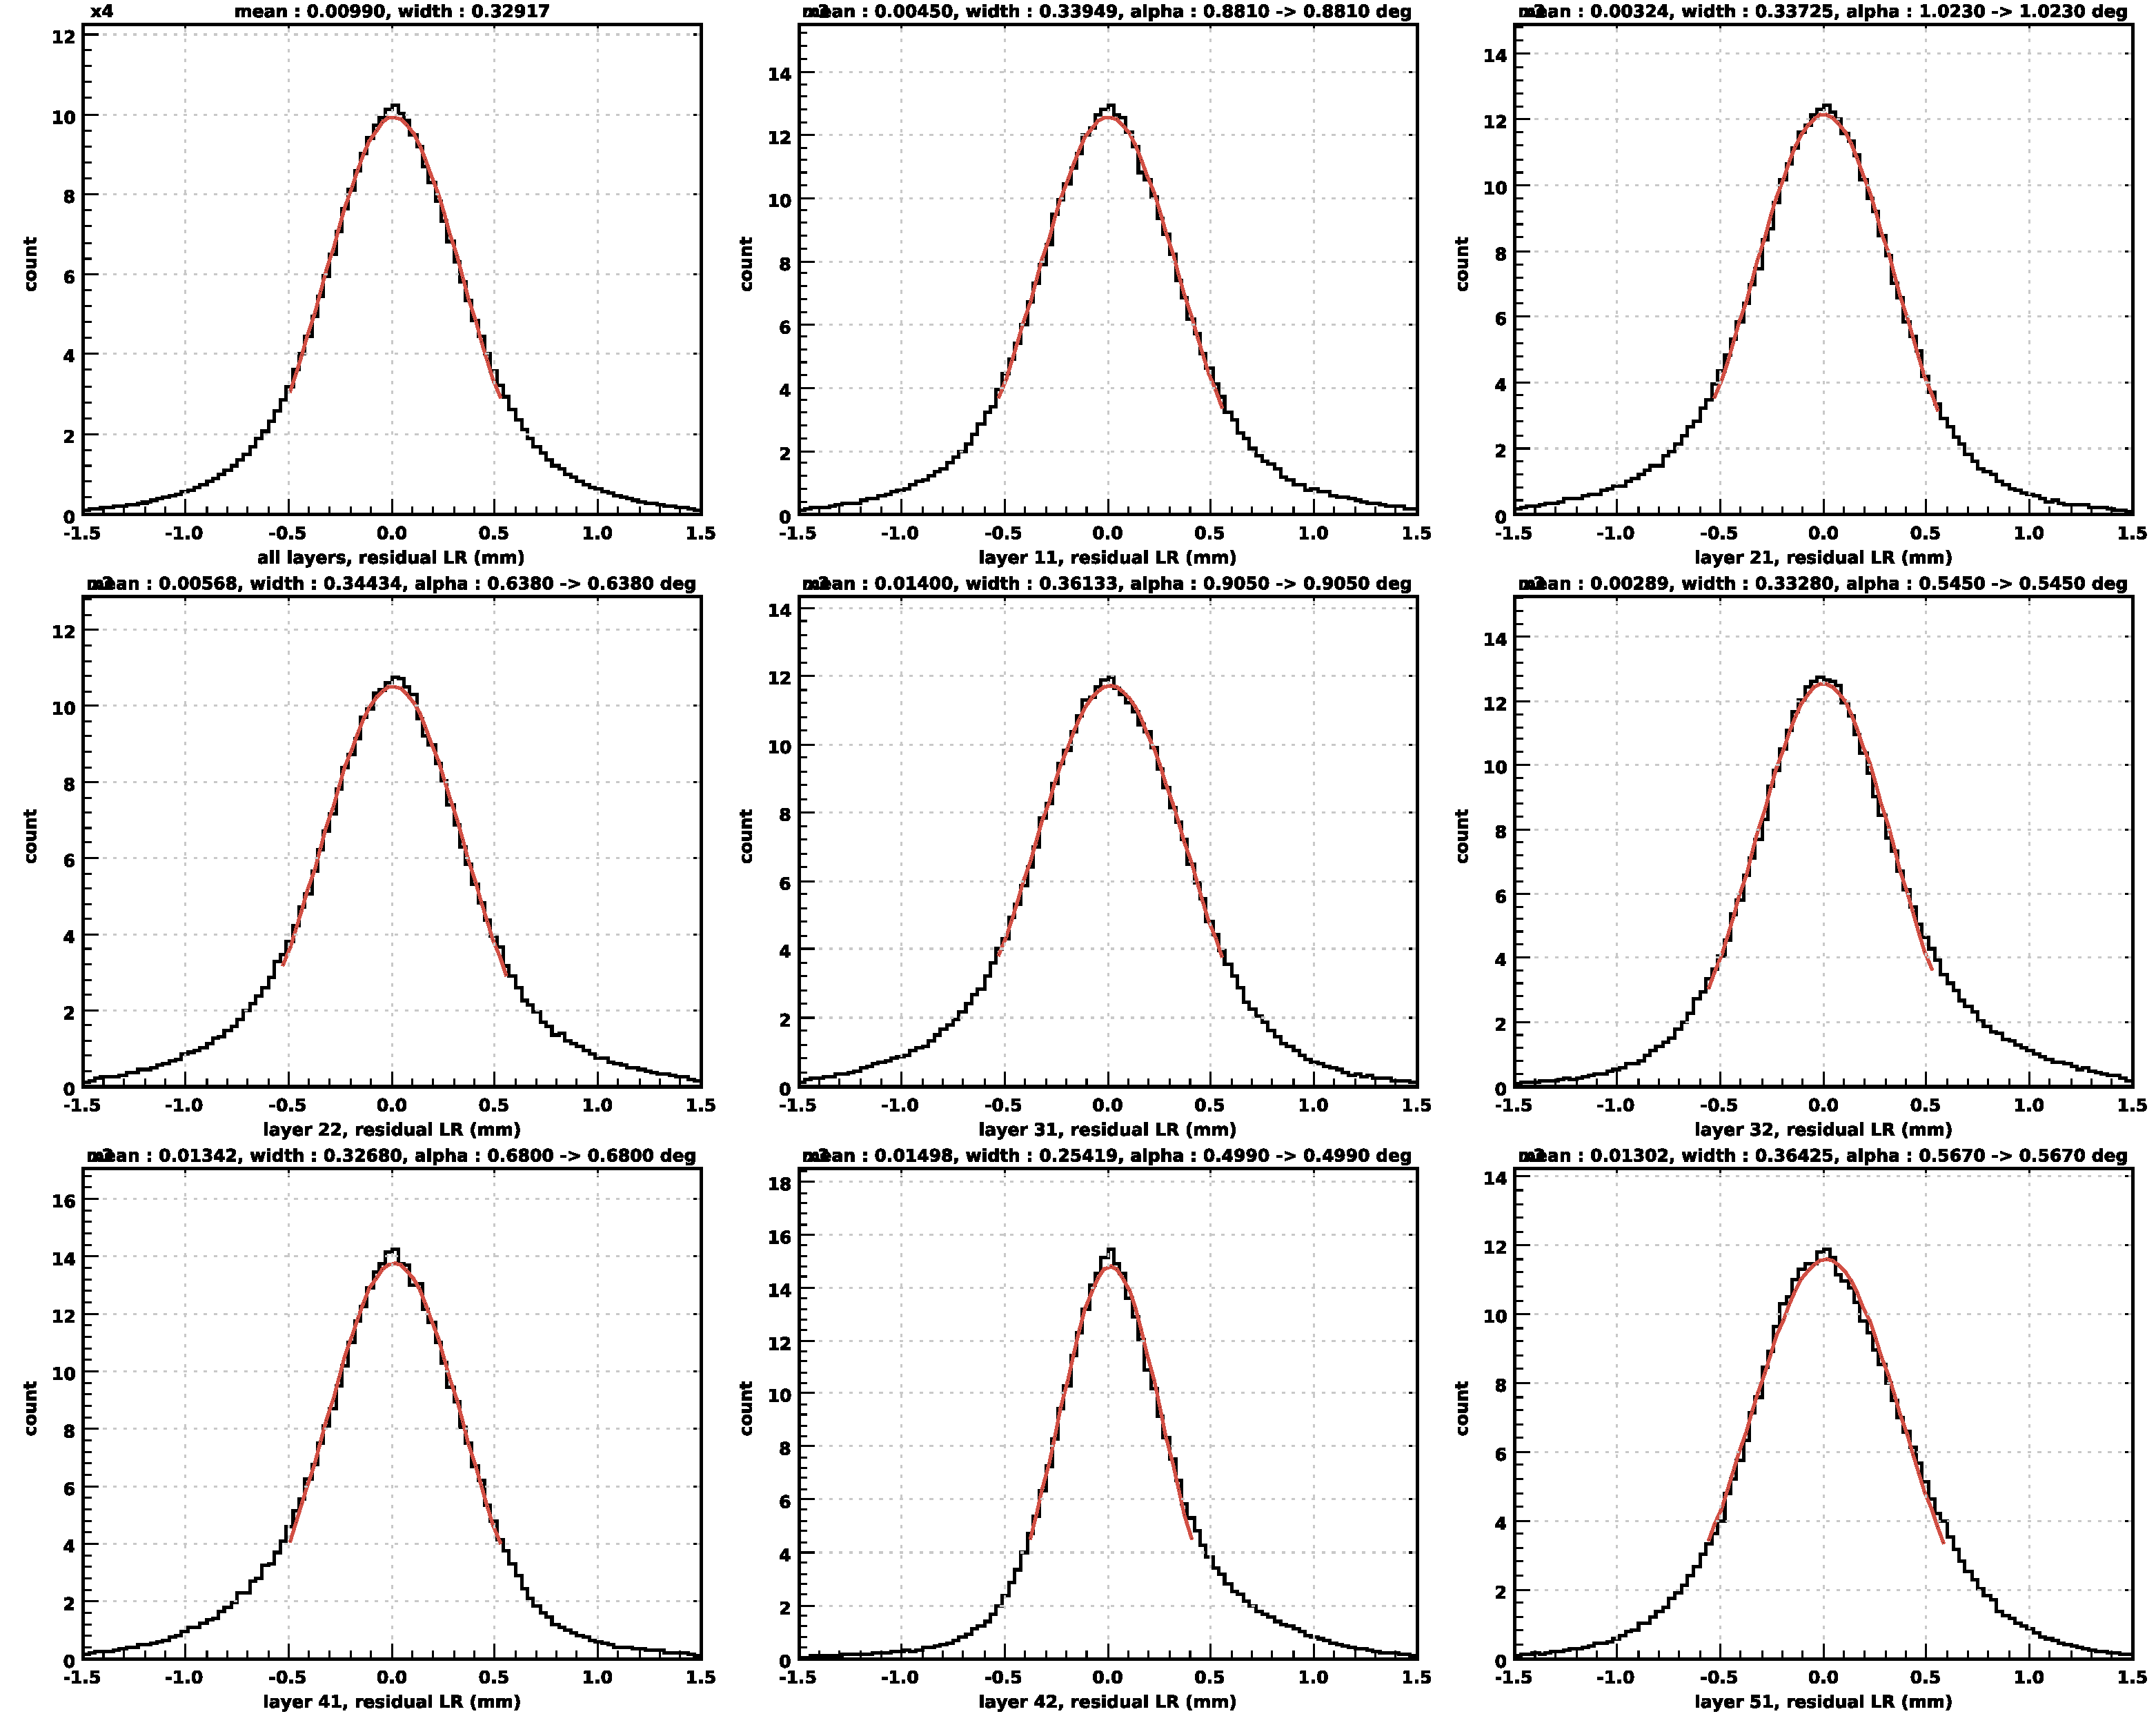
\includegraphics[width=\linewidth]{figures/cb_v12_residual_LR_iter_1.pdf}
    \end{minipage}
    
\end{frame}

\begin{frame}{Updates - layer alignment}
    \begin{itemize}
        \item Last week, I presented that after centering the integrated distribution, we still observed a vz dependence of the residual LR
        %\item At the end the minimize the 
    \end{itemize}

    \vspace{0.05cm}
    \centering
    \begin{minipage}{0.7\textwidth}
        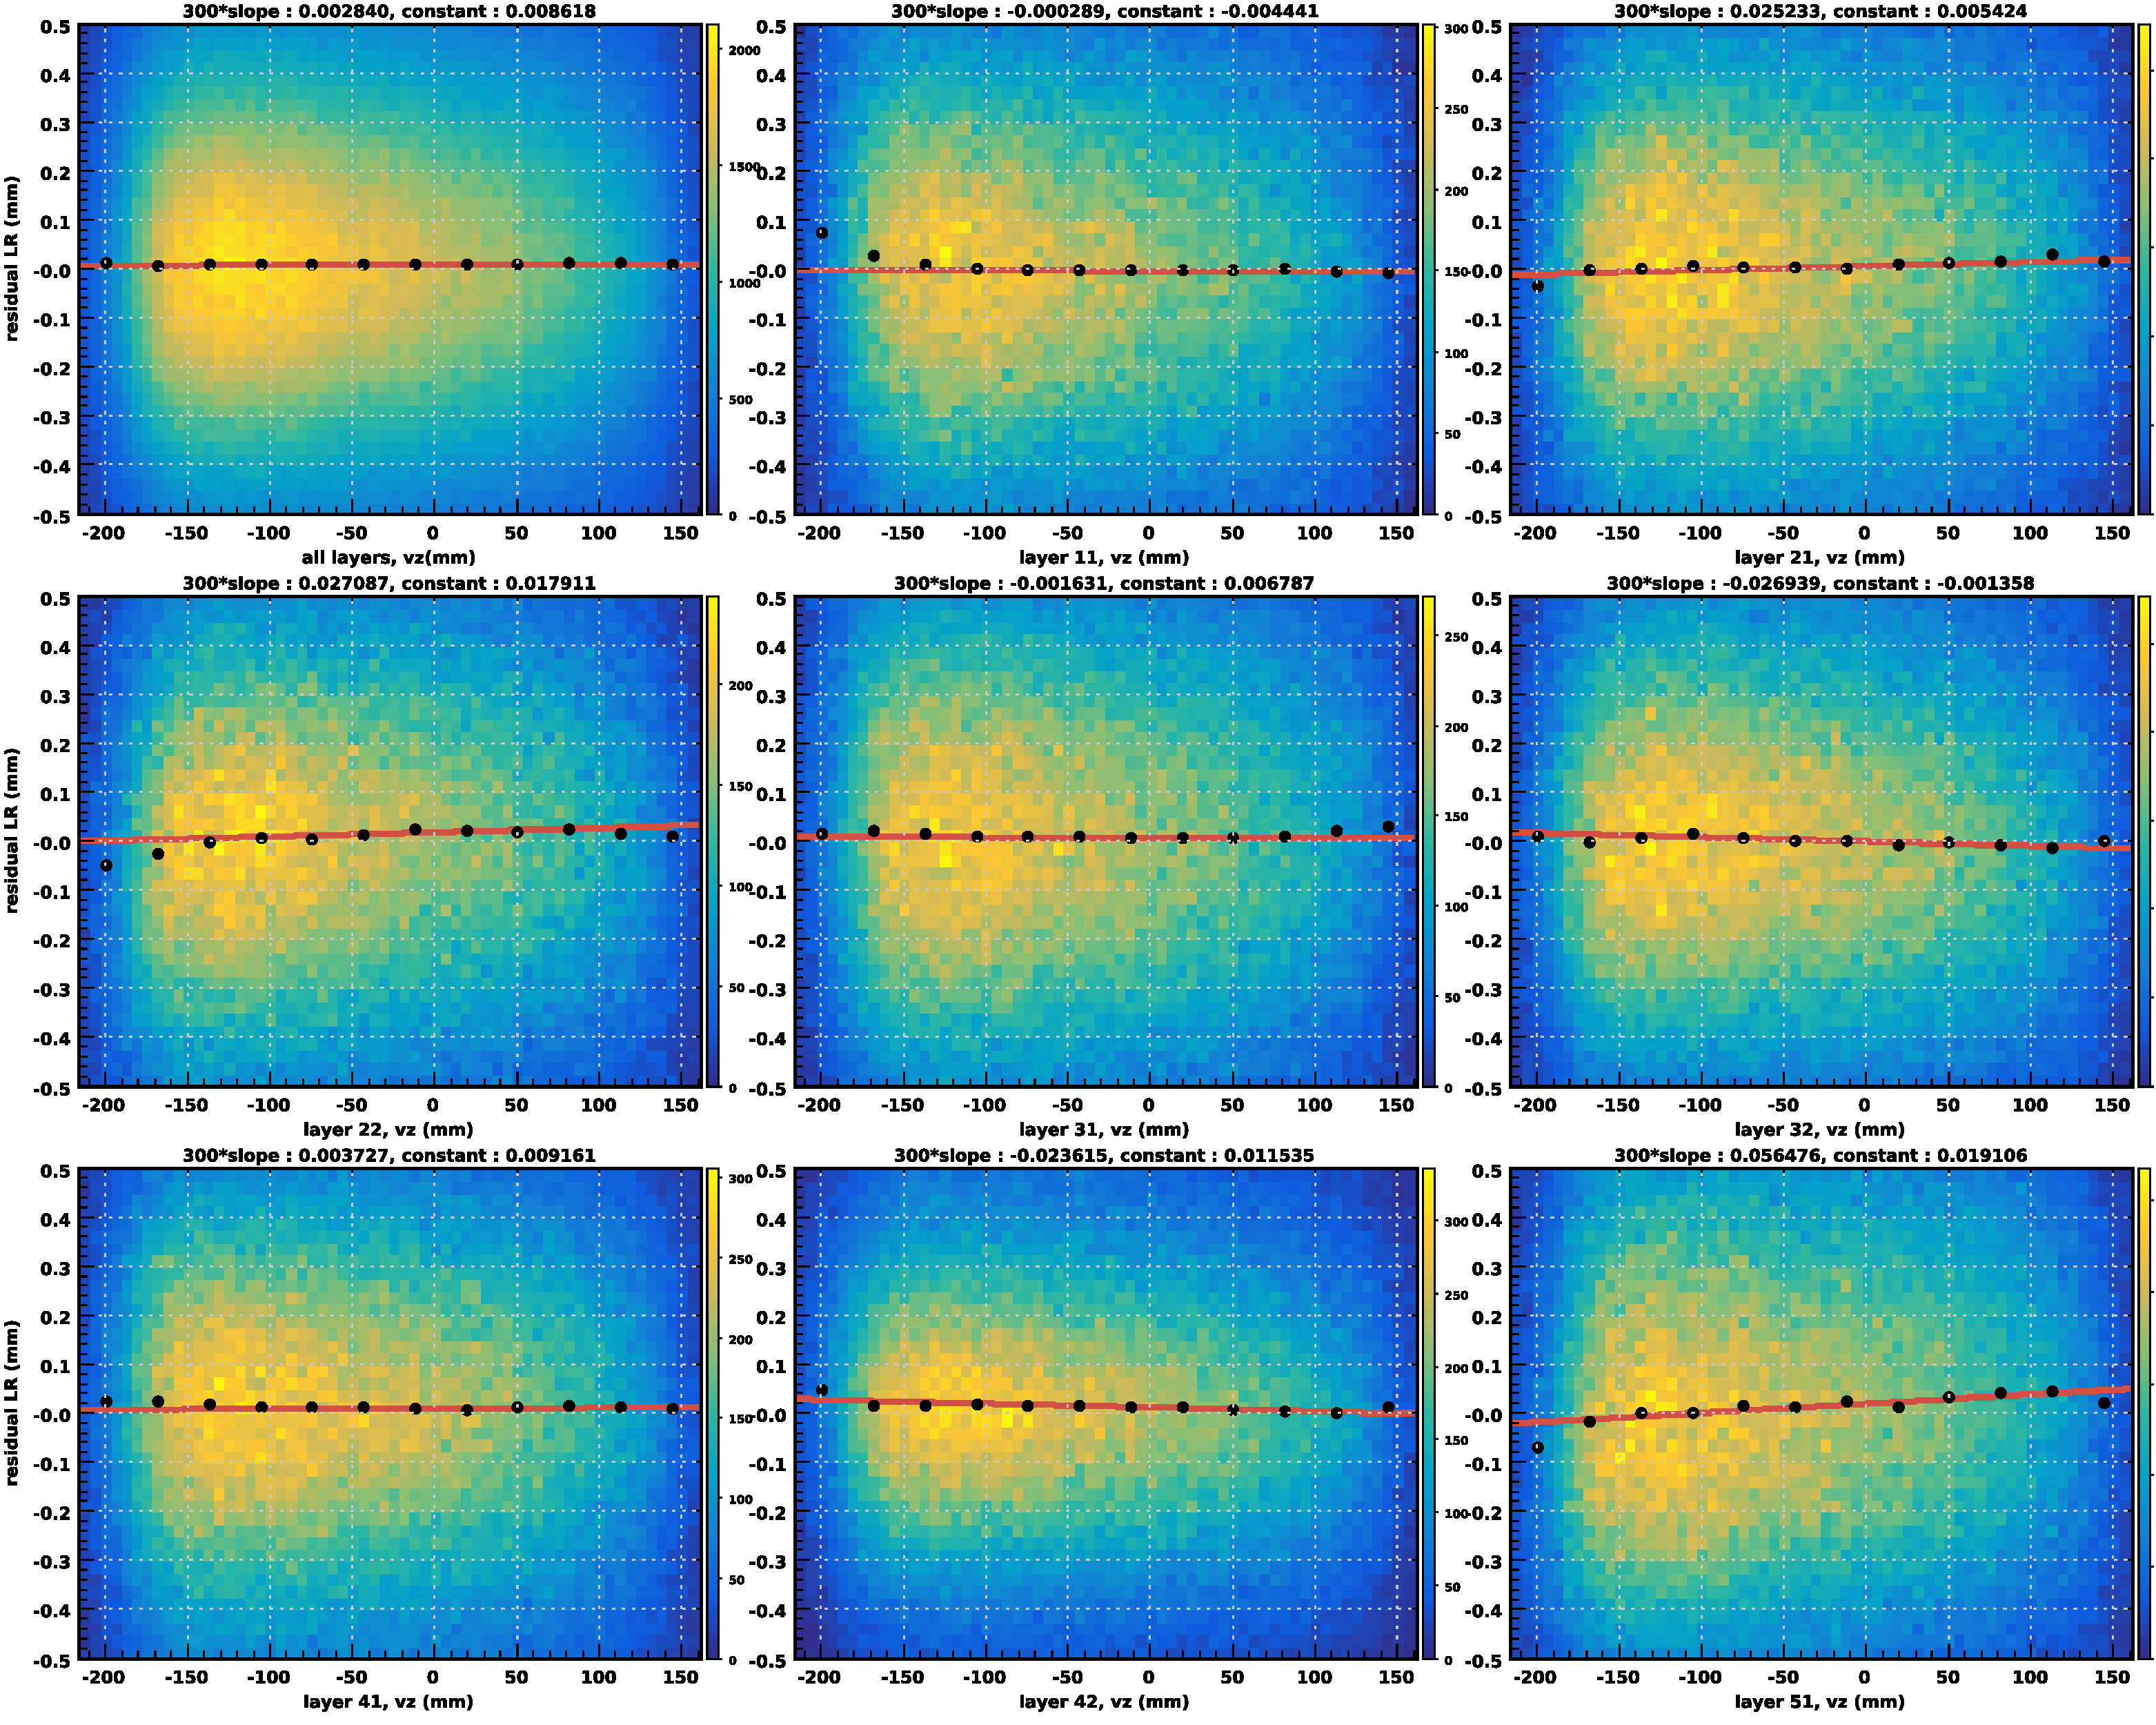
\includegraphics[width=\linewidth]{figures/cb_v12_corr_vz_residual_LR_iter_1.pdf}
    \end{minipage}
    
\end{frame}

\begin{frame}{Updates - layer alignment}
    \begin{itemize}
        \item This vz dependence gives us the idea that we should rotate the two points of the wire independently
        \item Here is the current approach
        
            \begin{enumerate}
                \item Fit the distribution
                    \[
                        r_i = a_0 + a_1 \cdot z
                    \]
                \item Estimate $r_i$ at $z = -188$ mm and $z = +162.5$ mm
                \item Compute correction angles at both end
                    \[
                        \alpha_i = \alpha_{i-1} - \frac{r_i}{R} \cdot \frac{1}{2}
                    \]
                \item Update AHDC geometry
            \end{enumerate}

    \end{itemize}

    
    \vspace{0.5cm}

    $r_i$ is the mean of the residual LR distribution\\
    $R$ is radius of the layer in which the wire belongs to
    
\end{frame}

\begin{frame}{Updates - layer alignment}
    \begin{itemize}
        \item Here is the redressed residual LR distribution versus the vz
        \item On layer 51, we moved from $300 \cdot $ slope = 0.05 to 0.006
    \end{itemize}

    \vspace{0.05cm}
    \centering
    \begin{minipage}{0.7\textwidth}
        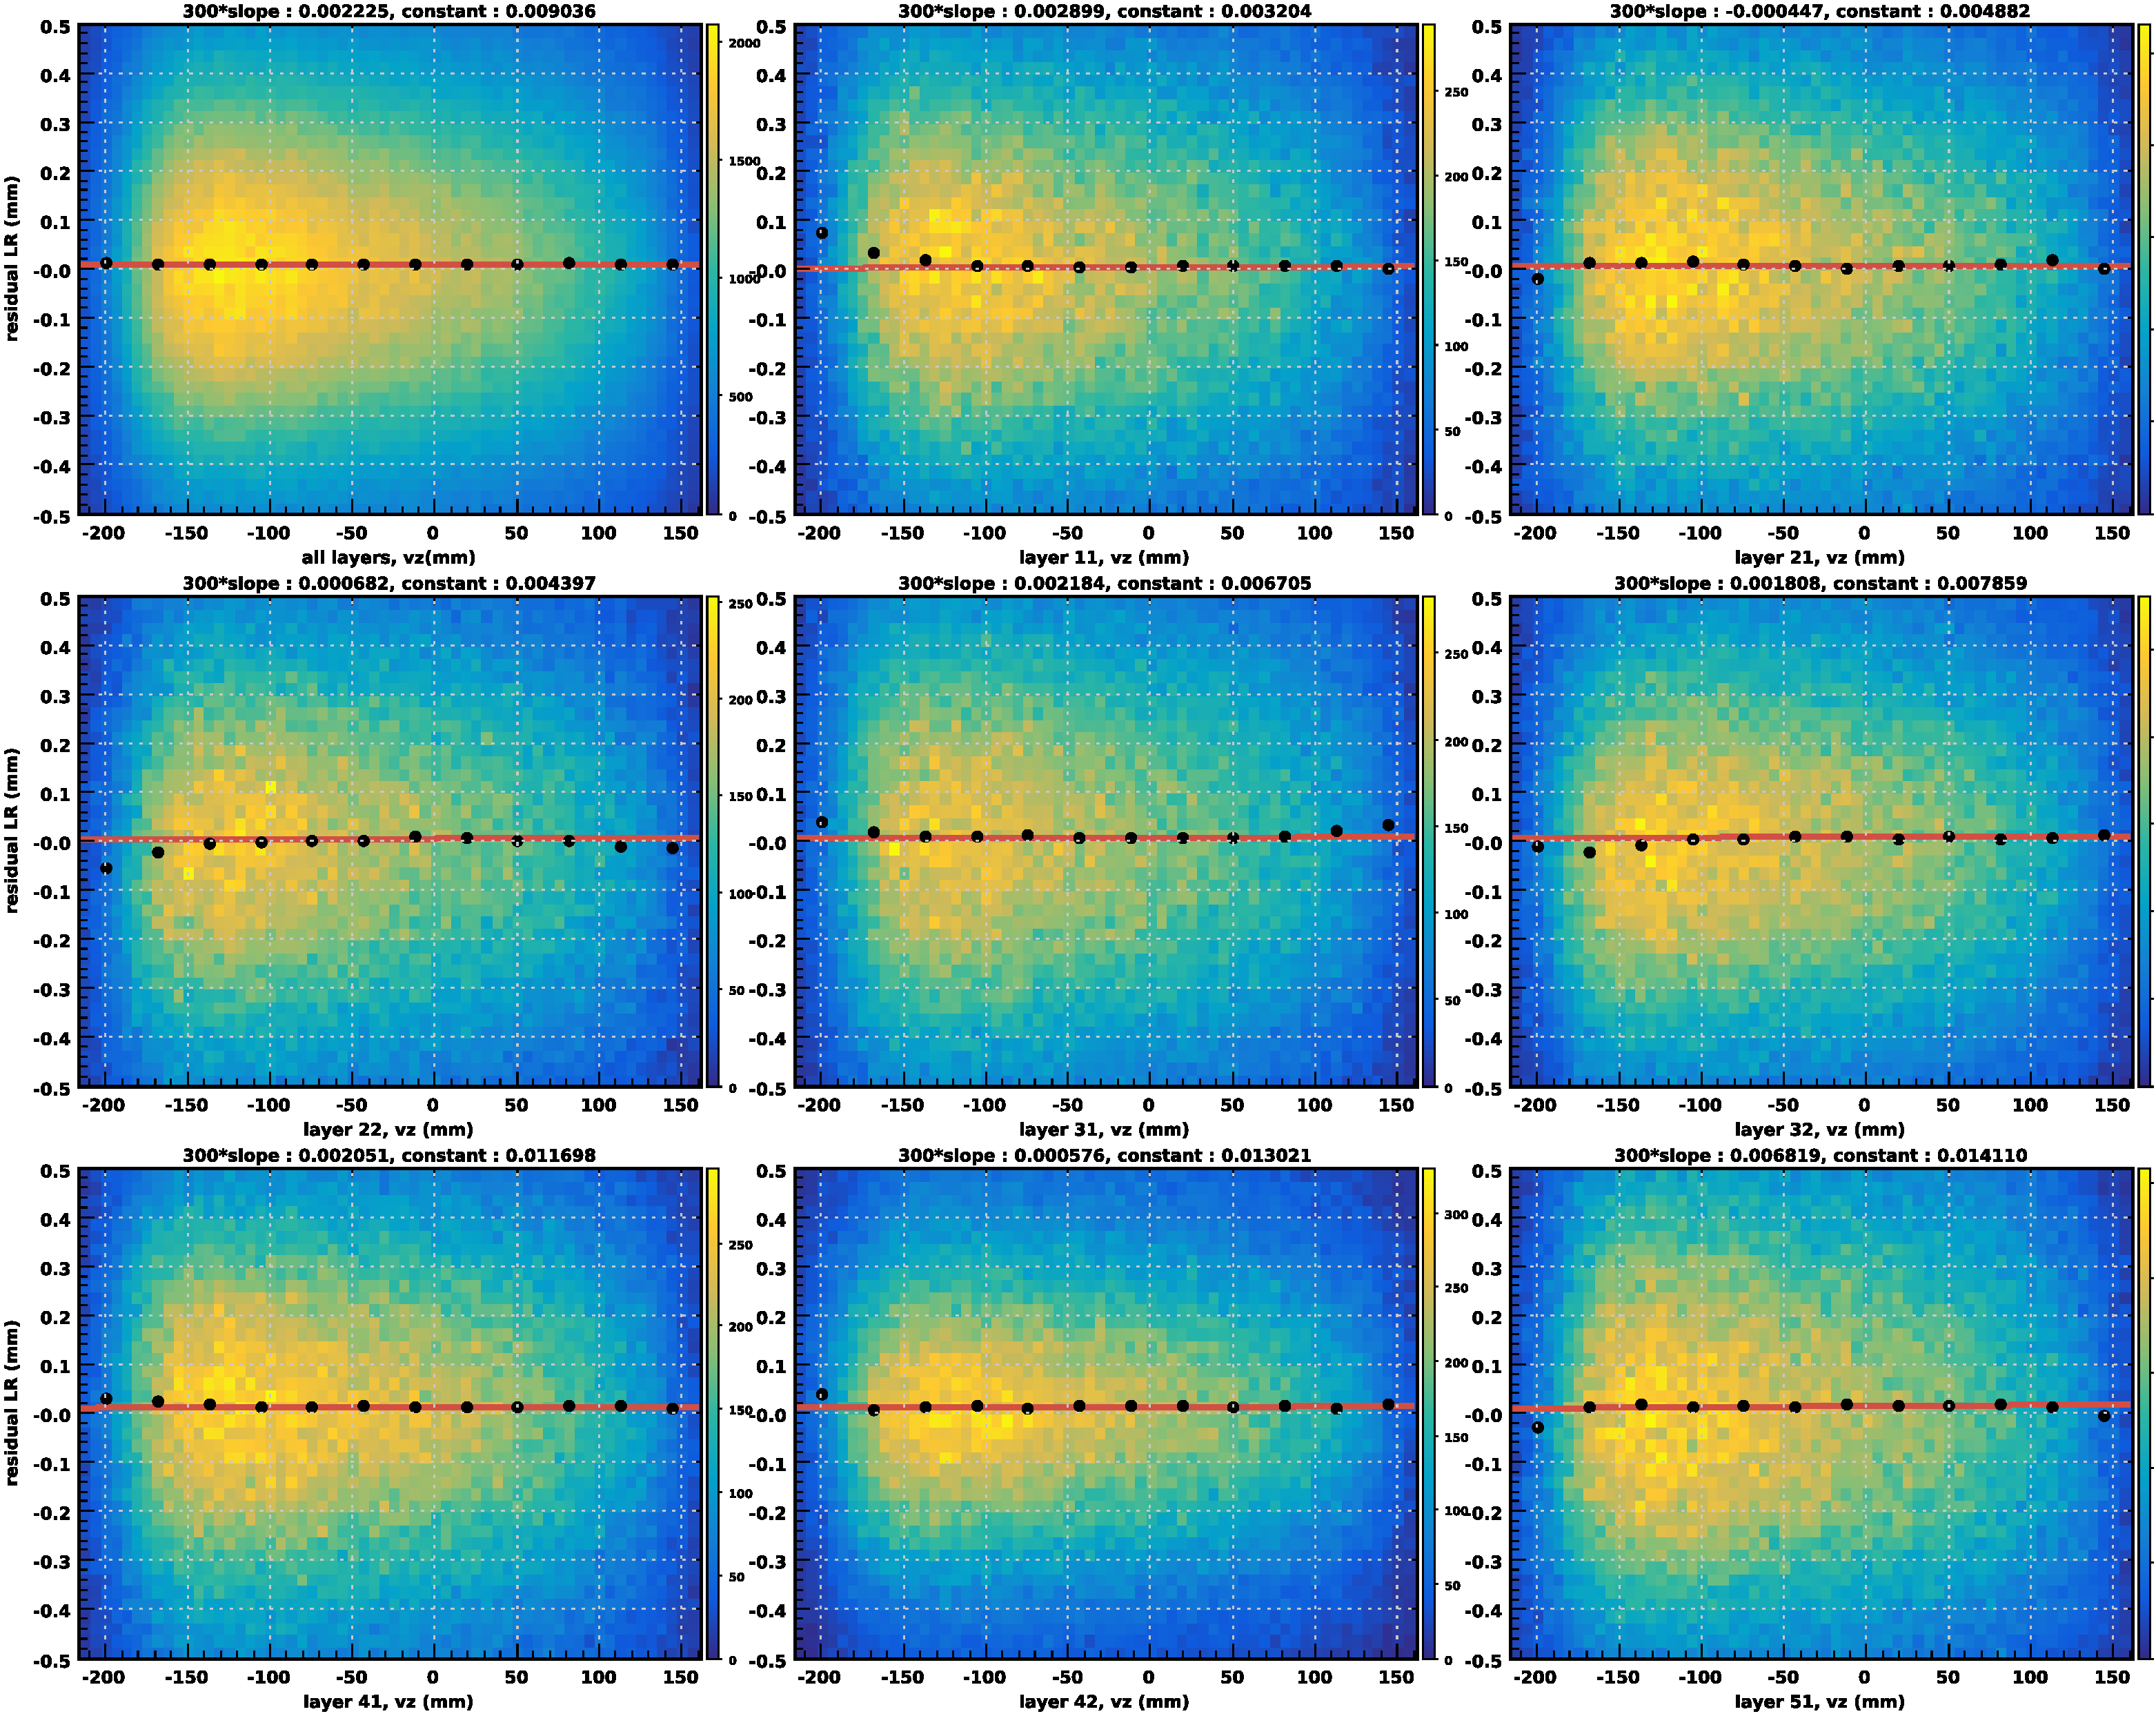
\includegraphics[width=\linewidth]{figures/cb_v13_corr_vz_residual_LR_iter_20.pdf}
    \end{minipage}
    
\end{frame}

\begin{frame}{Updates - layer alignment}
    \begin{itemize}
        \item Corresponding integrated distributions
        \item On layer 51, we moved from $300 \cdot $ slope = 0.05 to 0.006
    \end{itemize}

    \vspace{0.05cm}
    \centering
    \begin{minipage}{0.7\textwidth}
        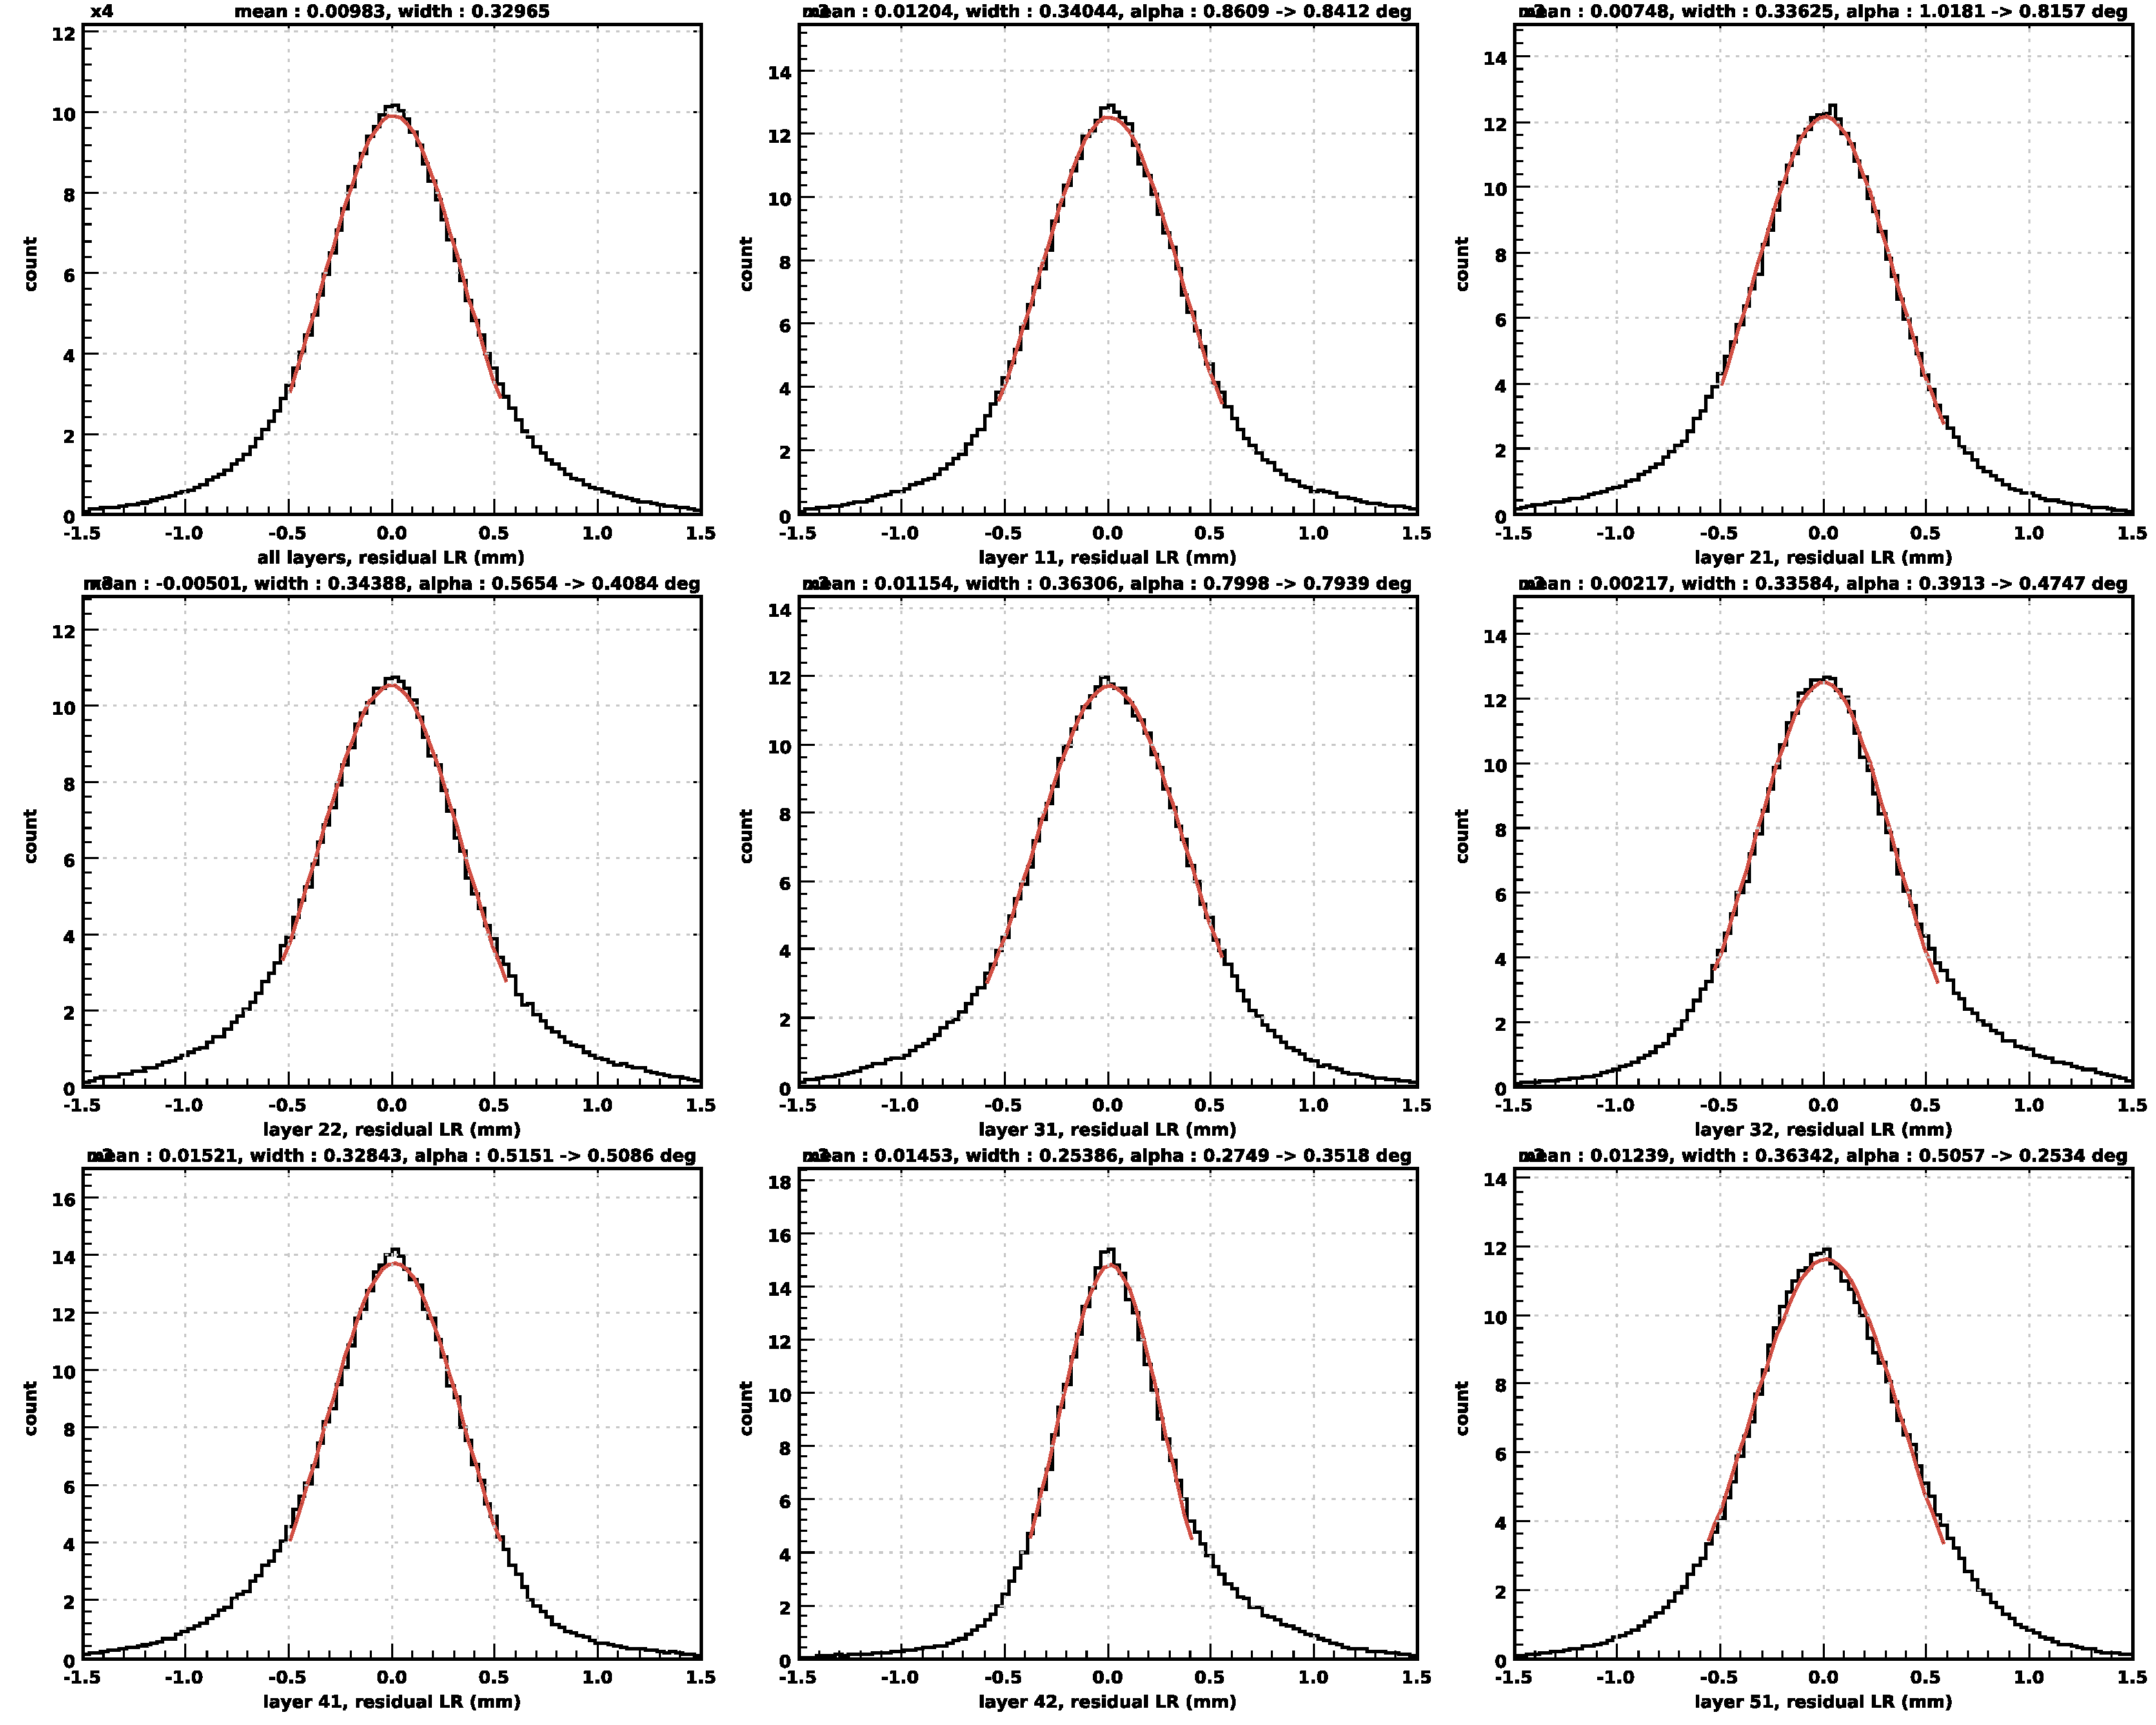
\includegraphics[width=\linewidth]{figures/cb_v13_residual_LR_iter_20.pdf}
    \end{minipage}
    
\end{frame}

\begin{frame}{Remark on the time2distance}
    \begin{itemize}
        \item Looking back at slide 2, we noticed the width of the residual LR distribution are not the same in each layer
        \item The layer 42 has the best width
       % \item 
    \end{itemize}

    \vspace{0.05cm}
    \centering
    \begin{minipage}{0.7\textwidth}
        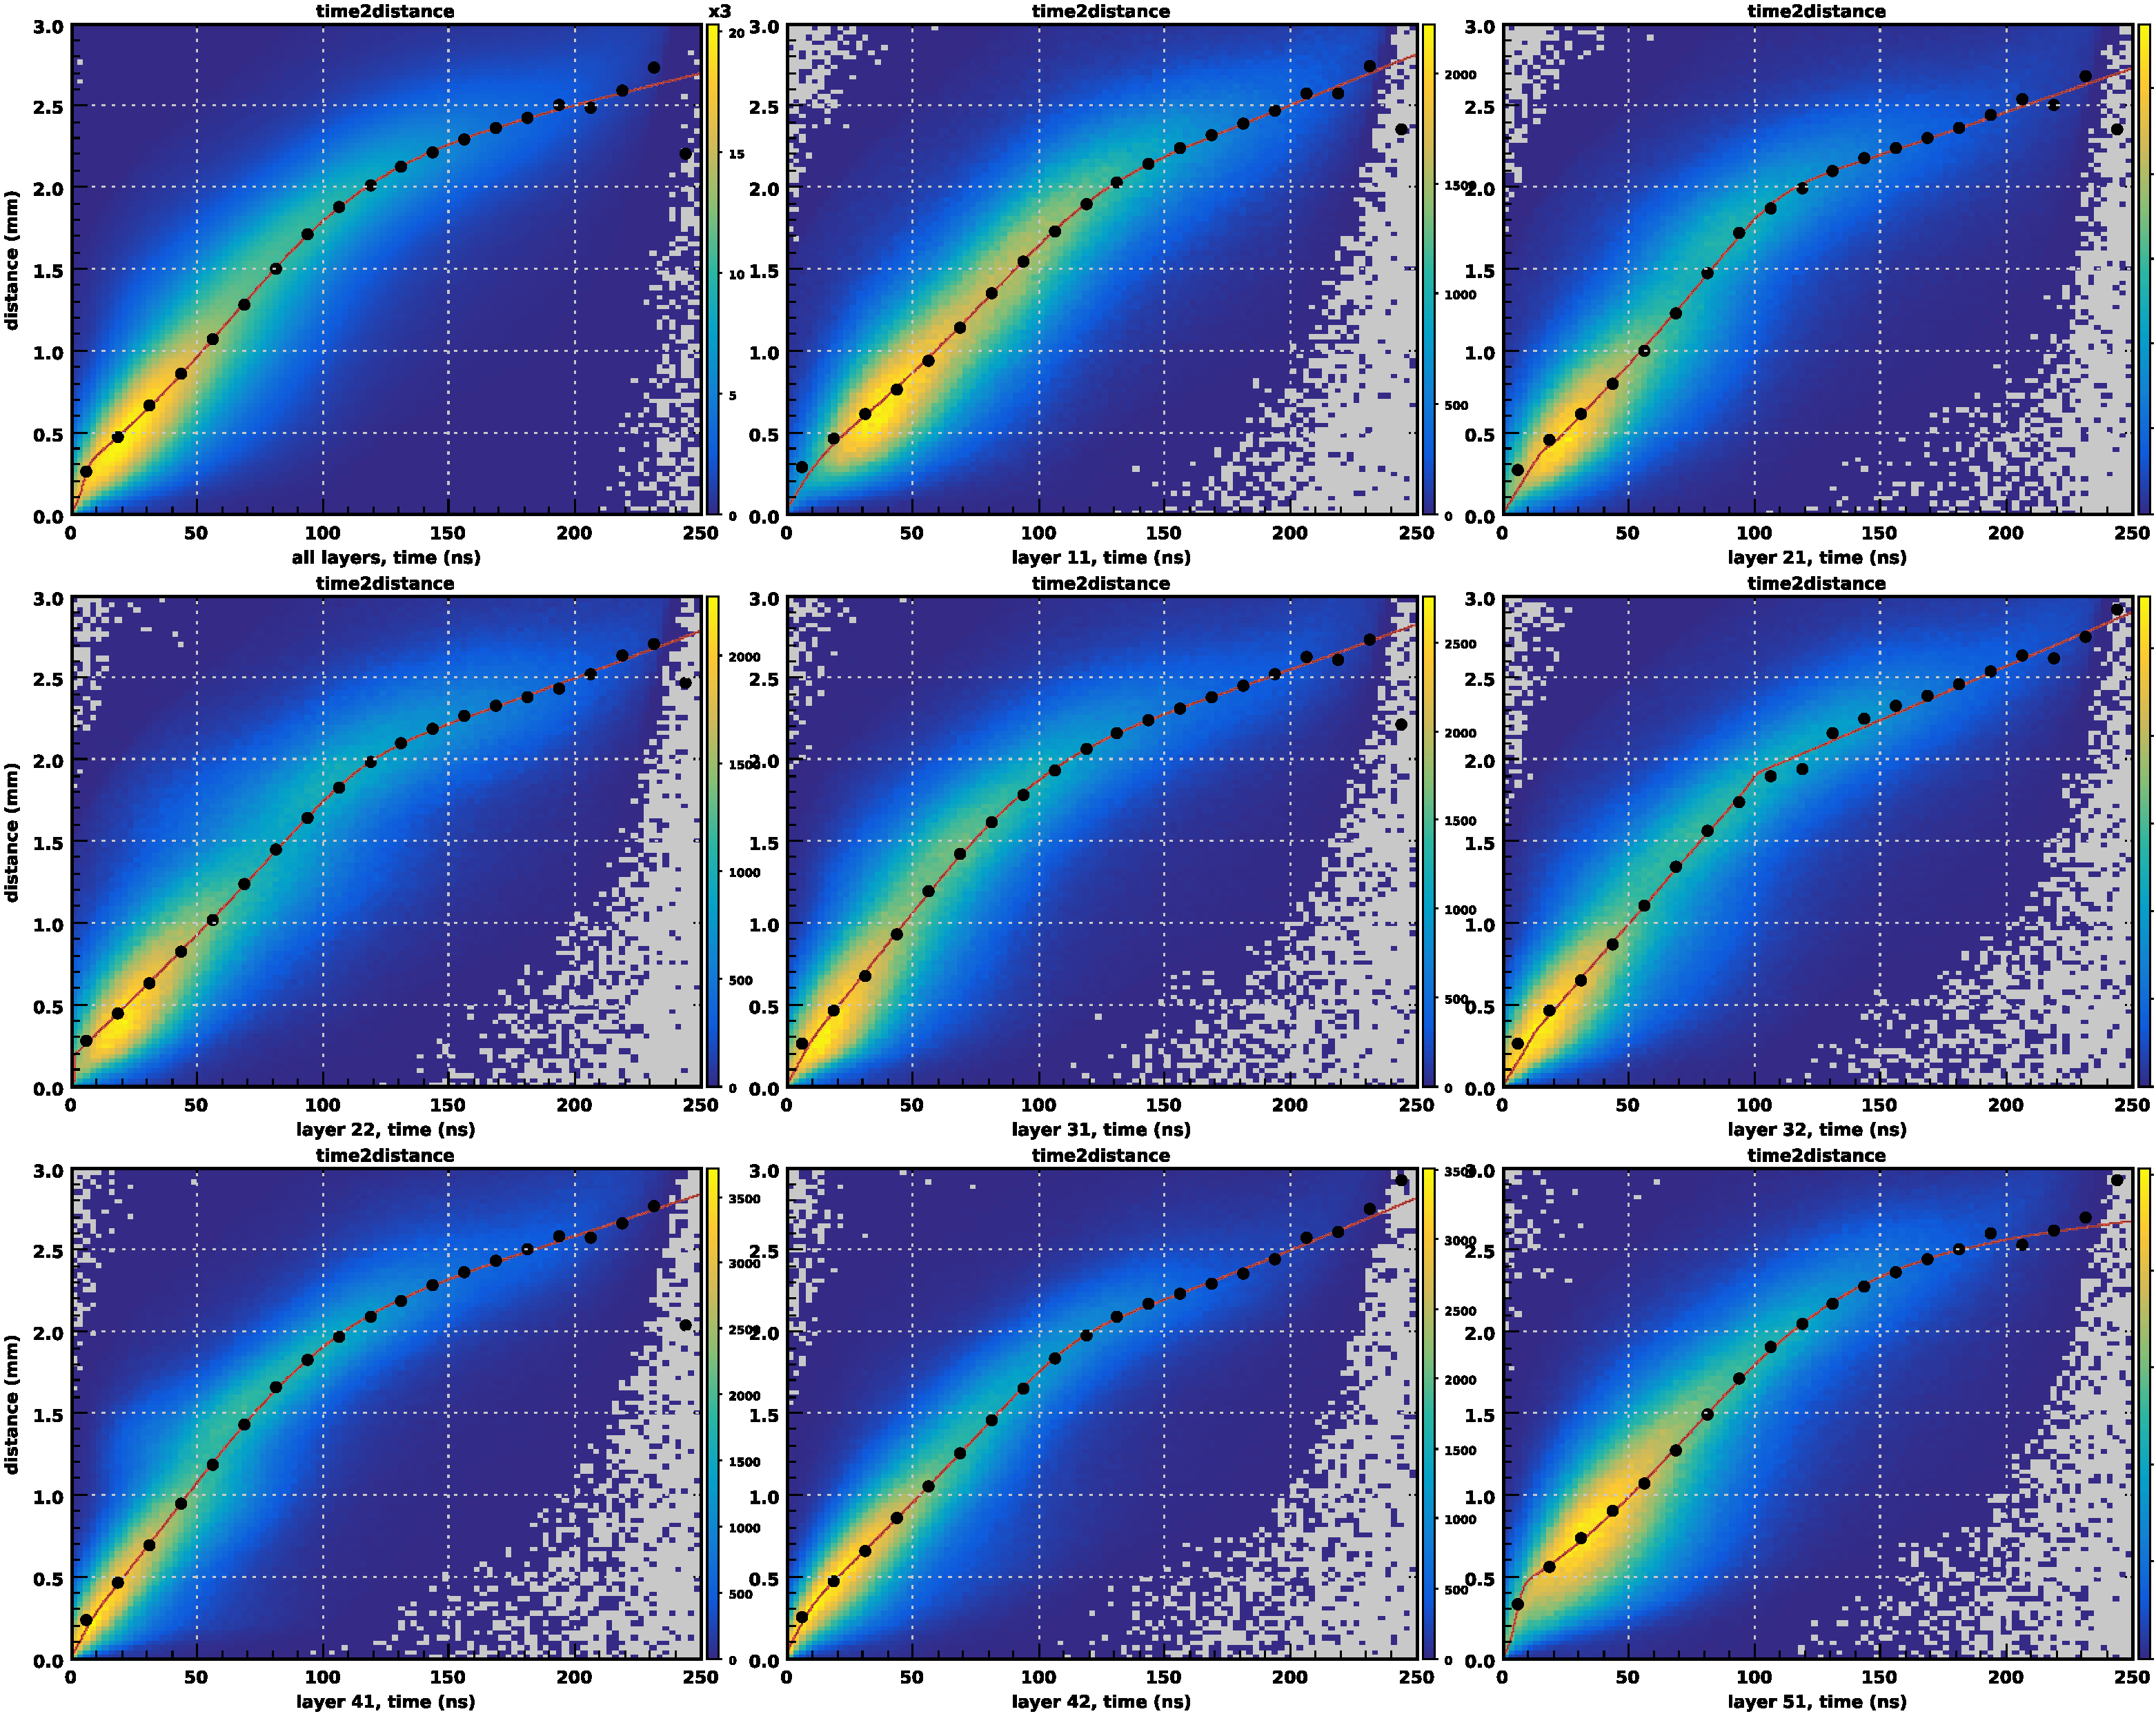
\includegraphics[width=\linewidth]{figures/time2distance_iter_1.pdf}
    \end{minipage}
\end{frame}

\begin{frame}{Remark on the time2distance}
    \begin{itemize}
        \item Fit parameters
    \end{itemize}

    \vspace{0.5cm}

    { \scriptsize

    {\color{red} \# parameters:} (p1\_int, p1\_slope, p2\_int, p2\_slope, p3\_int, p3\_slope, t1\_x0, t1\_width, t2\_x0, t2\_width, z0, z1, z2, extra1, extra2, chi2ndf)

    {\color{red} layer 11} 0.0   0.025   0.1524432438269216   0.013662109606346983   1.238888015143148   0.006292724661723682   10.61858511373951   7.294273613688368   111.90536249864928   19.46290697010042   0.0 0.0 0.0 0.0 0.0 0.0\\

    {\color{red} layer 21} 0.0   0.025   0.10593913807841789   0.01592833219948447   1.386583736836944   0.005362034573582515   16.860137333505854   1.2568118180267442   102.27327461156732   12.452719290020083   0.0 0.0 0.0 0.0 0.0 0.0\\

    {\color{red} layer 22} 0.0   0.025   0.16746410221131006   0.014752903877788583   1.3253408898127226   0.005837023064645656   1.3849664283500365   0.03595687486766891   109.27926538710621   17.05884016237542   0.0 0.0 0.0 0.0 0.0 0.0\\

    {\color{red} layer 31} 0.0   0.025   0.04182463535525476   0.017043148318961532   1.3692524424526162   0.0058054270340739044   6.935454981547715   2.625939342494976   86.80469951798632   28.90512489886573   0.0 0.0 0.0 0.0 0.0 0.0\\

    {\color{red} layer 32} 0.0   0.025   0.10544221513444453   0.017723302439479414   1.2475393438695748   0.006607858328105532   11.847536025587633   0.7453314294304595   99.77423252811073   1.0077423252811073   0.0 0.0 0.0 0.0 0.0 0.0\\

    {\color{red} layer 41} 0.0   0.025   0.007884490501318307   0.016326746295293498   1.5098443029064812   0.005304253505791621   7.148140463280074   2.68984043827601   80.53150804782068   29.528637561653127   0.0 0.0 0.0 0.0 0.0 0.0\\

    {\color{red} layer 42} 0.0   0.025   0.18632890517038658   0.015130215241519692   1.2147716093408516   0.006399341648561764   5.819193187447101   4.174336483250375   110.8479522545242   15.346634548147998   0.0 0.0 0.0 0.0 0.0 0.0\\

    {\color{red} layer 51} 0.0   0.024737567181385325   0.20610168381854832   0.004217131199467733   2.2927386517612725   0.001564434065283897   5.735501015758339   1.2865216784904034   80.43292637092915   34.01797963884968   0.0 0.0 0.0 0.0 0.0 0.0
    }

\end{frame}

\begin{frame}{Remark on the time2distance}
    \begin{itemize}
        \item To do the fit, I use the new T2D form proposed by Micheal
        \item We may have an issue in the formula implemented in coatjava
    \end{itemize}

    \[
        \mbox{T2D}(x) = (1-t_1)\cdot P_1 + t_1 \cdot (1-t_2) \cdot P_2 + {\color{red} t_1} \cdot t_2 \cdot P_3
    \]

    \[
        t(x) = \frac{1}{1+\exp\left(-\frac{x-x_0}{\sigma}\right)}
    \]

    \[
        P(x) = a_{0} + a_{1}\cdot x
    \]

    \vspace{0.05cm}
    \centering
    \begin{minipage}{0.4\textwidth}
        \includegraphics[width=\linewidth]{figures/build/time2distance_formula.pdf}
    \end{minipage}
\end{frame}

\begin{frame}{Next steps}
    \begin{itemize}
        \item I will continue my work on the alignment
            \begin{itemize}
                \item \sout{Rotate independently the two end points of the wires in a given layer}
                \item Push the study further by doing a wire by wire alignment
            \end{itemize}
        \item Pending task
            \begin{itemize}
                \item Push my work on the ATOF hits for the Kalman Filter in coatjava
                \item Finish the work on the Kalman Filter (material verification, target gas density, PID, magnetic field, optimization)
            \end{itemize}
    \end{itemize}
    
\end{frame}



\begin{frame}{Backup slides}
    \begin{itemize}
        \item Procedure:
            \begin{enumerate}
                \item We looked at elastic events : electron + track (here: collection of hits only)
                \item We computed the theoretical momentum vector of the track $\vec{p}$
                \item We made the propagation without doing any fit (i.e no KF correction)
                \item We looked at {\color{blue} residual\_LR} (left-right) $\longrightarrow$ sensitive to the alignment
            \end{enumerate}
    \end{itemize}
    

    \vspace{0.2cm}
    \centering
    \begin{minipage}{0.42\textwidth}
        \includegraphics[width=\linewidth]{figures/build/illustration_residual_type.pdf}
    \end{minipage}

\end{frame}






\end{document}


